%\input{capitulos/metodo}
\chapter[Materiais e Métodos]{Materiais e Métodos}
\label{cap_Materiais e Metodos}

    No presente capítulo será tratado a classificação e o delineamento da pesquisa. Também serão exploradas cada etapa de desenvolvimento do protótipo do sistema proposto.
    
%\section{Delineamento da pesquisa}
%\label{subsec_Delineamento da pesquisa}

    Com base nas definições expostas por \citeonline[Cáp.~4]{turrioni_2012_metodologia}, a presente pesquisa pode ser classificada segundo a natureza, objetivo, abordagem e método. Quanto a \textit{natureza}, esta é uma pesquisa aplicada devido ao caráter prático da solução, que se baseia em explorar o uso de sensores de baixo custo para detecção das dimensões de bagagens. Quanto ao \textit{objetivo}, a pesquisa é exploratória, visto que, busca analisar a capacidade de uso dessa tecnologia para a tarefa citada. Sobre a \textit{abordagem}, é uma pesquisa quantitativa, que busca comparar os resultados obtidos com a tecnologia proposta aos resultados das dimensões reais. Em relação ao \textit{método}, é entendido que a pesquisa desenvolvida tem caráter experimental e de simulação computacional, devido ao objetivo de criação e avaliação de modelos e protótipos. 
    
    Ainda, conforme o modelo de classificação disponível pelo conselho Nacional de Desenvolvimento Científico \cite{cnpq_2022_engenharias}, este projeto pode ser classificado em 3 subtópicos. Quanto a engenharias, o subtópico é "Equipamentos Auxiliares e Controles" dado que o produto contribui com o controle no processo de check-in. O segundo é o subtópico de “desenvolvimento de produto” do tópico de engenheira de produção, visto que será construído um protótipo para validar os resultados com chances de dar origem a um produto. Quanto a ciências exatas e da terra é o subtópico de Arquitetura de Sistemas de Computação, uma vez que é desenvolvido um sistema embarcado para automação das partes físicas do projeto. A seguinte árvore ilustra os tópicos citados:
    
\dirtree{%
.1 Engenharias.
.2 Engenharia de Transportes.
.3 Veículos e Equipamentos de Controle.
.4 Equipamentos Auxiliares e Controles.
.2 Engenharia de Produção.
.3 Engenharia do Produto.
.4 Desenvolvimento de Produto.
.1 Ciências Exatas e da Terra.
.2 Ciência da Computação.
.3 Sistemas de Computação.
.4 Arquitetura de Sistemas de Computação.
}\label{tree:Árvore de classificação da presente pesquisa} 
    



%\section{Desenvolvimento do modelo para obtenção de dimensões de bagagens}
%\label{sec_Desenvolvimento do modelo para obtenção de dimensões de bagagens}

    Tendo exposto o delineamento dessa pesquisa, cabe avançar para explicação do desenvolvimento da solução. Sendo assim, visando explorar a efetividade técnica do uso de equipamentos de baixo custo na detecção de dimensões de bagagens, foi desenvolvido um protótipo. Para tanto, foi adotada uma metodologia de desenvolvimento baseada em fases sequenciais e retroativas com melhoria sucessiva dos modelos e/ou algoritmos mediante testagem e feedbacks. Esse fluxo foi inspirado em métodos tal como Cascata e Scrum, cuja as descrições podem ser encontradas em \cite{bourque_2015_guide}. A Figura \ref{fig:fluxogramaModeloPropostoObtencaoDimensoes} mostra o modelo geral para obtenção das dimensões das bagagens proposto por essa pesquisa.


        \begin{figure}[h]
           \centering
           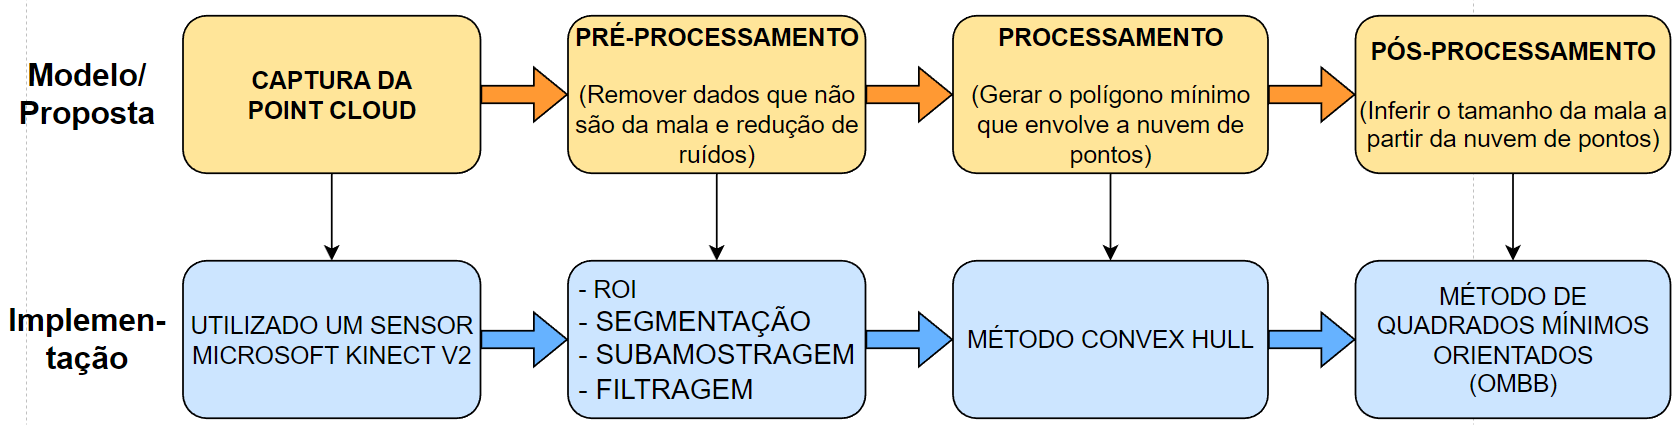
\includegraphics[width=1\textwidth]{imagens/fluxogramaModeloPropostoObtencaoDimensoes.png} 
           \caption{Fluxograma do modelo proposto para obtenção de dimensões}
          \label{fig:fluxogramaModeloPropostoObtencaoDimensoes}
        \end{figure}

    O fluxo ilustrado na Figura \ref{fig:fluxogramaModeloPropostoObtencaoDimensoes} consiste em 4 fases. A primeira etapa é a captura dos dados, para a qual foi construído um dispositivo físico. Na segunda etapa, a \textit{point cloud} é tratada para retirada de ruídos. A terceira etapa consiste em obter os pontos de borda com o convex hull. Na última etapa é obtida as dimensões pelo uso de OMBB. Foram avaliados fatores tais como, custo, tempo de medida, posição do sensor, posição das bagagens e exatidão. Ao longo do texto, são relatadas as dificuldades de implementação e complexidade de incorporação do sensor. 
    
    Quanto a estrutura do protótipo, este, deve comportar bagagens de mão e de despacho. Para captura da \textit{point cloud} foi escolhido o sensor de profundidade kinect v2. Isso é devido a seu baixo custo (alinhado com a proposta da pesquisa) e sua alta precisão, dados discutidos na Seção \ref{sec_Fundamentacao_teorica}.
    
    Para o desenvolvimento dos códigos foi escolhido utilizar o MATLAB \cite{mathworks_2019_matlab}, devido a existência de drivers para interação com o sensor e bibliotecas para manipulação da \textit{point cloud}. Para a automação das partes estruturais, foi utilizado o Arduino, devido a praticidade e quantidade de módulos disponíveis para automação de dispositivos. As próximas seções detalham os módulos desenvolvidos para a solução.



\section{Captura da \textit{Point Cloud}}
\label{subsec_Captura da Point Cloud}


    O primeiro passo do modelo proposto consiste em obter a \textit{point cloud}. Para tanto, foi desenvolvido um dispositivo utilizando o sensor de profundidade kinect v2. O equipamento consegue mover as bagagens através do campo de ação do sensor que captura os pontos da superfície da mala. O sistema realiza esse processo tendo como parâmetros uma região de captura, frequência de amostragem, passo e velocidade da esteira. Para tanto, as dependências que dão suporte ao Kinect v2 no MATLAB utilizadas nessa pesquisa foram as seguintes: 

    \begin{itemize}
        \item Image aquisiton toolbox: kit para aquisição de dados por meio de alguns dispositivos (câmera, raio-x, Kinect etc) \cite{mathworks_2022_image};
        \item Image Acquisition Toolbox Support Package for Kinect For Windows Sensor: pacote com drives necessários para comunicar o sistema com o kinect v1 ou v2 \cite{mathwork_2022_image};
    \end{itemize}
    
    Os recursos disponíveis para o kinect, permitem a obtenção de \textit{point clouds} com cores ou sem cores. A sem cores é chamada de “\textit{Only depth}”, sendo gerada em um menor tempo de processamento que a colorida, esse foi o tipo utilizado nessa pesquisa. Tais dados são reunidos em um Objeto \textit{point cloud}, este, tem as principais propriedades da amostra sendo elas a matriz de pontos (x, y, z) em unidade de metros, matriz de pontos RGB, matriz de intensidade em escala de cinza, número de pontos e limites do plano. 
    
    Duas funcionalidades disponíveis para o Kinect e importantes para a solução em questão são a região de interesse (ROI) e a subamostragem. O ROI permite retornar pontos em um limite definido por um vetor contendo as coordenadas de largura, comprimento e altura da região, isso possibilita a delimitação do campo de captura de dados. A subamostragem permite reduzir a densidade de pontos da \textit{point cloud} original, isso contribui com a otimização do tempo de processamento em etapas posteriores \cite{mathworks_2015_point,mathworks_2017_acquire}. As seções seguintes detalham a implementação do protótipo.


\subsection{Modelagem da solução para captura da \textit{point cloud}}
\label{subsubsec_Modelagem da solucao}

    Após os testes dos componentes do sistema, foram avaliadas as abordagens para captura e manipulação da \textit{point cloud}. Assim como outros sistemas de visão computacional, na presente pesquisa existem 3 etapas gerais, sendo a captura dos dados, tratamento da \textit{point cloud} e extração dos dados de dimensões. Na primeira etapa foram avaliadas as formas de captura da \textit{point cloud}, sendo elas a captura estática e a móvel. 


%\subsubsubsection{Amostragem de point cloud de forma estática}
%\label{subsubsubsec_Amostragem de point cloud de forma estática}

    A captura estática consiste em posicionar o sensor em um ponto fixo e coletar a \textit{point cloud} de um objeto abaixo. Sendo assim, foi escolhida a posição Topo (90°) mostrada na Figura \ref{fig:posicoesSensorProfundidade}. Essa abordagem foi utilizada em trabalhos tal como \cite{gao_2013_baggage} e \cite{qingji_2018_method} porém sem o uso do kinect. Nesse tipo de amostragem, é simulado o caso do passeiro colocar a mala em um ambiente estático (sem esteira), a bagagem é medida e ele retira a mesma do local. O modelo que ilustra esse processo é mostrado na Figura \ref{fig:amostragem de point cloud de forma estatica}.
    
        \begin{figure}[h]
           \centering
           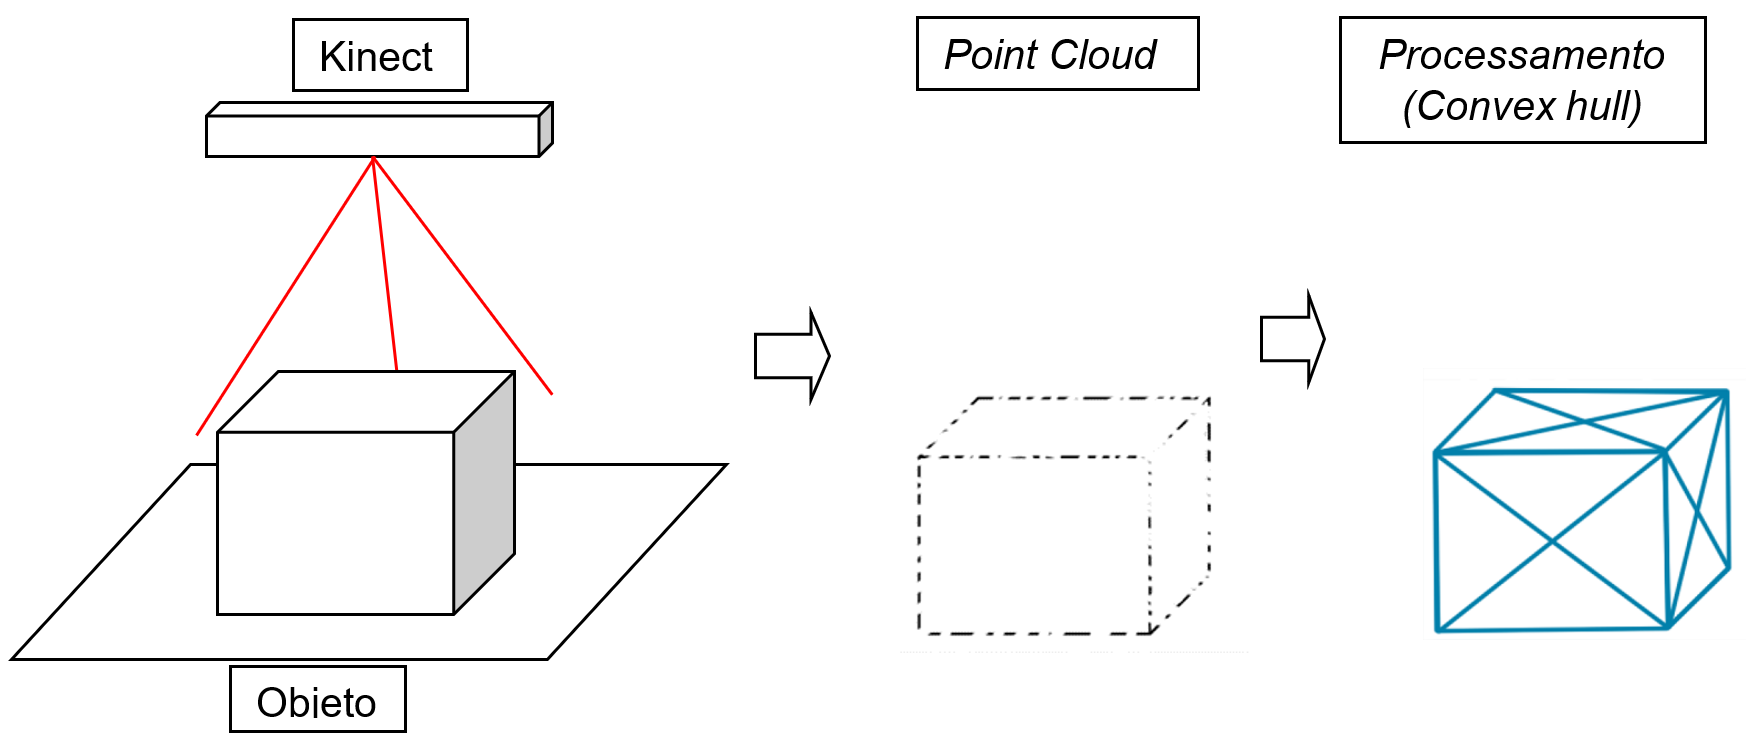
\includegraphics[width=0.8\textwidth]{imagens/amostragemEstaticaPtCloud.png} 
           \caption{Amostragem de \textit{point cloud} via sensor kinect}
          \label{fig:amostragem de point cloud de forma estatica}
        \end{figure}

    A posição do sensor tem influência nos resultados e no método para obtenção das dimensões. Por exemplo, com apenas um sensor, a visão lateral de 90° que detectá pontos diretos de uma face da mala, poderia ter oclusão de dados, gerando erros caso a mala tenha um comprimento e/ou formato diferente do lado ocluso. Nesse caso, teria que ser adicionada uma fase extra de tratamento para redução dessa oclusão via, por exemplo, espelhamento. A Figura \ref{fig:posicoesSensorProfundidade} indica quais as posições mais comuns observadas na revisão da literatura. 
    
        \begin{figure}[h]
           \centering
           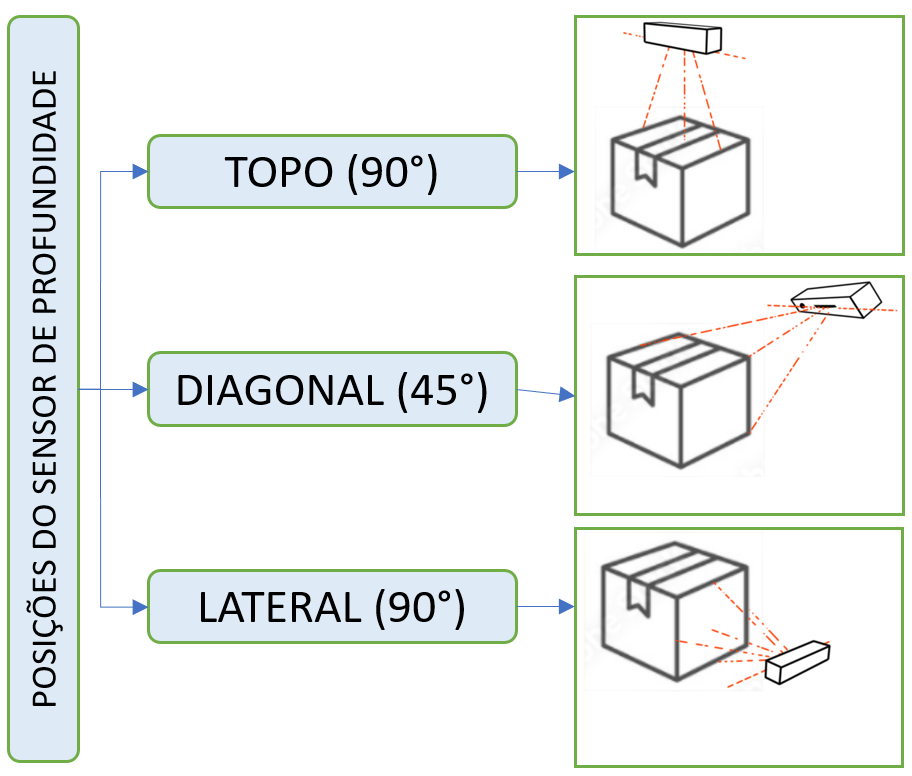
\includegraphics[width=0.45\textwidth]{imagens/posições do sensor de profundidade.png} 
           \caption{Posições mais comuns para o sensor}
           \label{fig:posicoesSensorProfundidade}
        \end{figure}

    Prosseguindo, a visão Topo (90°) foi selecionada, pois, na presente aplicação, reduz a quantidade de pontos oclusos aumentando o nível de detalhes capturados, como alças e deformações. Dado que é utilizado apenas 1 sensor, as demais posições tem maior chance de ocorrência de oclusão, reduzindo a quantidade de dados coletados das laterais da mala. Para fixação do Kinect e realização do primeiro teste, foi construída uma estrutura mostrada na Figura \ref{fig:Estrutura para testes com kinect}.

        \begin{figure}[h]
           \centering
           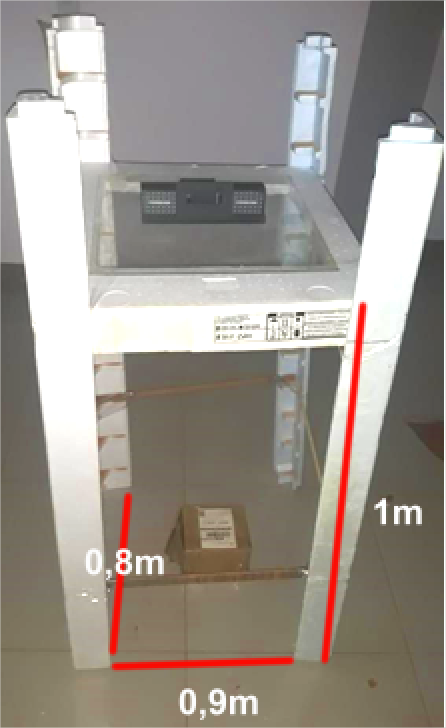
\includegraphics[width=0.3\textwidth]{imagens/EstruturaDeFixacaoKinectSemEsteira.png} 
           \caption{Estrutura de testes com kinect para amostragem estática}
          \label{fig:Estrutura para testes com kinect}
        \end{figure}
    
    
    
    Como pode ser visto na Figura \ref{fig:Estrutura para testes com kinect}, o Kinect foi posicionado na parte superior, a 1 metro da base, apoiado sobre um vidro. As laterais da estrutura estão distanciadas por 0,9 m de largura e 0,8 m de comprimento, totalizando uma área ativa de $0,72 m^2$.
    
    Para validação do cenário foi utilizado o Kinect studio com o propósito de visualizar a \textit{point cloud}. A Figura \ref{fig:cenarioTeste1}, mostra a reconstrução da superfície do cenário em 3D, já com a aplicação do ROI (\textit{region of interest}). Este, é um processo de segmentação onde os pontos fora de uma área definida em termos de largura, comprimento e profundidade são descartados.
    
        \begin{figure}[h]
           \centering
           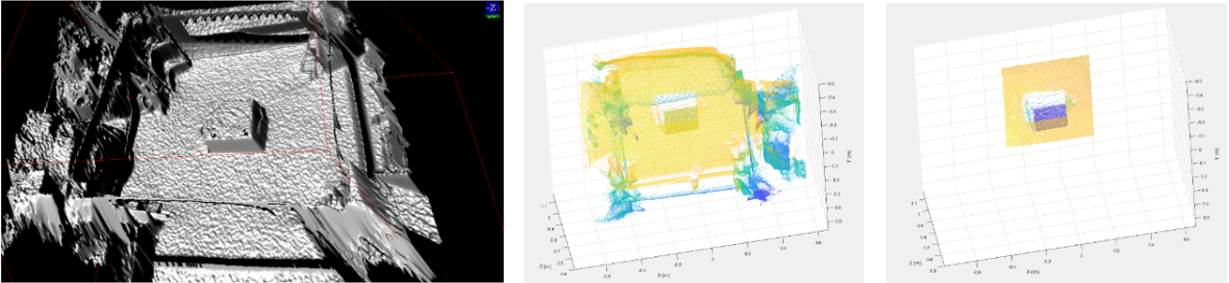
\includegraphics[width=1\textwidth]{imagens/cenarioTeste!.png} 
           \caption{Cenário de teste com reconstrução visual, \textit{point cloud} com região de interesse (roi) = 40 cm x 40 cm x 50 cm}
          \label{fig:cenarioTeste1}
        \end{figure}
    
    A captura estática consegue coletar a \textit{point cloud} com riqueza de detalhes. Porém, dado que os tamanhos/quantidade das bagagens são variáveis, não cobre todos os casos, como de bagagens maiores que a área ativa. Uma alternativa seria expandir essa área até o ponto que cobrisse todos os casos permitidos nos aeroportos, mas é um gasto desnecessário de recurso e poderia reduzir a serializarão dos testes com várias bagagens. Por isso, essa abordagem foi utilizada apenas como uma alternativa de aplicação do protótipo. 
    

%\subsubsubsection{Modelagem do protótipo físico para amostragem móvel}
%\label{subsubsubsec_Modelagem do protótipo físico para amostragem móvel}

    Diferente do modo estático, a captura móvel não tenta prever o tamanho das bagagens. Nesse caso, é definido um \textit{slice} que corresponde ao ROI de captura, passo de amostragem e uma frequência de amostragem. Essa abordagem consiste em se posicionar o sensor em um ponto fixo e mover o objeto pela região de ação do mesmo.
    
    Dado o comportamento da captura móvel, foi desenvolvido um protótipo.  Para tanto, foi acrescentado ao sistema uma esteira, capaz de mover uma bagagem através da região de amostragem do sensor. A Figura \ref{fig:ModeloPrototipoFisico} ilustra a ideia do protótipo, composta pelos passos a seguir:
    
    \begin{enumerate}
        \item O sensor permanece capturando dados e verificando a presença de um objeto dentro da região alvo;
        \item A central de controle representada pelo Arduino move o objeto acionando um motor que gira uma esteira;
        \item O objeto atravessa o campo de visão do sensor;
        \item A \textit{point cloud} é capturada em fatias (\textit{slices}), que são unidas em um só conjunto.
    \end{enumerate}


        \begin{figure}[h]
           \centering
           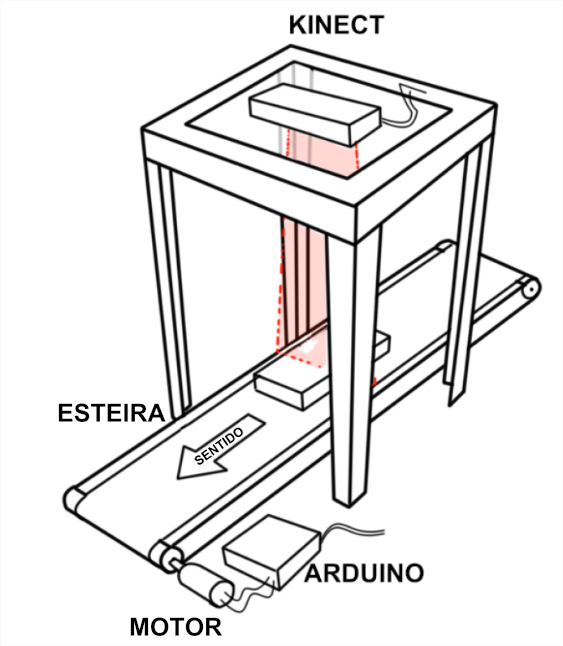
\includegraphics[width=0.45\textwidth]{imagens/ModeloPrototipoFisico.png}
           \caption{Modelo do protótipo físico para obtenção de dimensões de bagagens}
          \label{fig:ModeloPrototipoFisico}
        \end{figure}
    
    Como o objetivo final é trabalhar com o sistema em aeroportos, onde o cenário das bagagens é dinâmico, esta foi a abordagem selecionada para a construção do protótipo. Em próximas seções esse método será detalhado.
    

\subsection{Desenvolvimento do hardware e algoritmo de captura de dados}
\label{subsubsec_Desenvolvimento do hardware do protótipo}

    Esta subseção trata do desenvolvimento do protótipo físico. Este, foi baseado no modelo mostrado na Figura \ref{fig:ModeloPrototipoFisico}. Serão expostos os pontos principais quanto as medidas, central de controle, montagem e algorítimos utilizados. 
    
%\subsubsubsection{Medidas da esteira e posição do sensor}
%\label{subsubsubsec_Medidas da Esteira e posição do sensor}

    Quanto as medidas, foi constatado via teste que o alcance mínimo do sensor é aproximadamente 0,5 m com um erro de $\pm{0,06}$ em média. Esse erro pode ser originário da reflexão do sensor na superfície do objeto, ou mesmo de imprecisões no dispositivo. Isso significa que essa é a distância mínima para coleta de dimensões, tendo influência no produto final desta pesquisa, já que as partes físicas estarão limitadas ao campo de ação do sensor. Por tanto, a altura mínima adequada para o sensor, na posição topo 90°, é 1 m. 
    
    Dado que existem limites para que a esteira comporte as bagagens, foi seguido a medida máxima para bagagens de despacho, o que permite inserir também bagagens de mão, essas dimensões são  informadas na Seção \ref{subsec_processo Processo de embarque}. Com isso, as laterais da estrutura têm $0,7 m$ de largura e $1,10 m$ de comprimento (área total de $0,77 m$) com o sensor posicionado, por padrão, a $1 m$ de altura. Também foi considerada uma tolerância de $20 cm$ a mais para cada medida. 
    
    Com isso, foi construída uma estrutura de fixação para o Kinect que pode ser acoplada na esteira, a Figura \ref{fig:prototipoEsteira} mostra o resultado. Como citado, a posição selecionada para o sensor foi a topo 90° que reduz o número de pontos oclusos, aumentando o nível de detalhes como alças, etiquetas, deformações, objetos presos a mala e rodas. 


%\subsubsubsection{Desenvolvimento da central de controle}
%\label{subsubsubsec_Desenvolvimento da central de controle}



    A construção da esteira consistiu em duas partes, sendo a primeira o desenvolvimento do algoritmo a ser gravado no Arduino para central de controle e a segunda, a construção do hardware da esteira. A modelagem e simulação do circuito foram feitas no Proteus \cite{proteus_2022_pcb}, um sistema para simulação de circuitos. A Figura \ref{fig:EsquemaDoCirtuitoDaCentralDeControle}, mostra o modelo gerado e os componentes utilizados. Mais detalhes da implementação estão no Apêndice \ref{apend_Códigos fonte do sistema de médida de bagagens}.
    
        \begin{figure}[h]
           \centering
           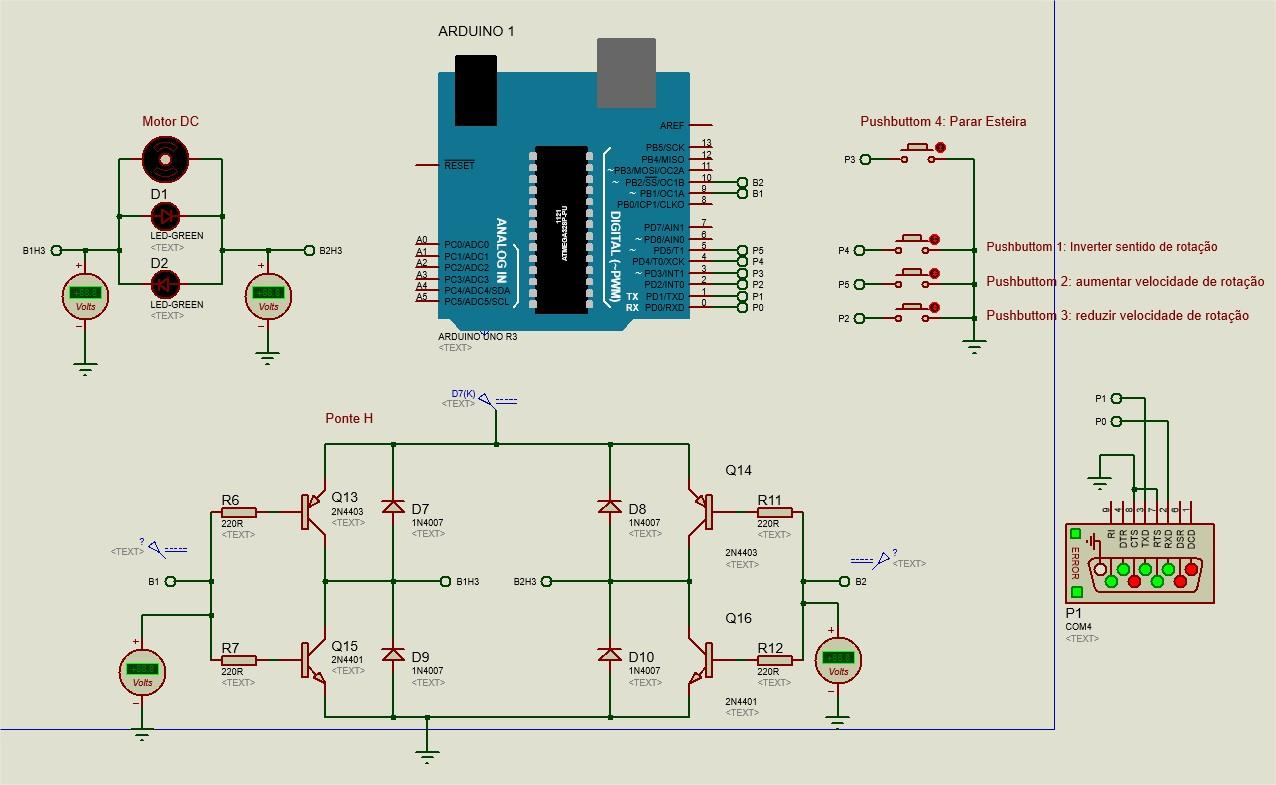
\includegraphics[width=1\textwidth]{imagens/EsquemaDoCirtuitoDaCentralDeControle.png}
           \caption{Simulação do Circuito da Central de controle da esteira}
          \label{fig:EsquemaDoCirtuitoDaCentralDeControle}
        \end{figure}
    
    Na Figura \ref{fig:EsquemaDoCirtuitoDaCentralDeControle} é possível visualizar a presença dos módulos do circuito. O Arduino é o microcontrolador e a Ponte H permite o controle isolado do motor, possibilitando inversão de sentido e controle da velocidade por PWM (pulso com modulação - \textit{pulse width modulation}). Também foi implementado um controlador feedback em malha fechada para ajustar o RPM (Rotações por minuto) do motor.  O Motor DC movimenta o tapete da esteira, sendo este de 12 V e pelo menos 4 A. No código, o PWM é controlado por um valor entre 0 e 255. A equivalência é de 1 para 0,00211 m/s. As opções de controle da esteira podem ser acessadas via porta serial, interface mostrada no Apêndice \ref{apend_Interface de usuário} ou por botões, sedo elas as seguintes:
    
    %O Algoritmo desenvolvido está disponível no Github\footnote{https://github.com/Vitor0534/CodigoPrototipoEsteira}. 
    

\begin{itemize}
    \item Push button 1: controle do sentido de rotação, horário ou anti-horário;
    \item Push button 2: aumentar a velocidade de rotação. Permite até cinco velocidades, sendo elas (sem carga):
    \begin{itemize}
        \item Velocidade 1: $0m/s$; 
        \item Velocidade 2: $0,0895m/s$; 
        \item Velocidade 3: $0,205m/s$; (Padrão)
        \item Velocidade 4: $0,352m/s$;
        \item Velocidade 5: $0,538m/s$.
    \end{itemize}
    \item Push button 3: reduzir velocidade da esteira, até 0m/s;
    \item Push button 4: botão de emergência que para a esteira por meio de uma interrupção.
\end{itemize}

    Partindo para etapa de montagem do circuito, após testes fora da esteira, este foi colocado em uma caixa para proteção. A Figura \ref{fig:CentralDeControleEsteira} mostra o sistema fora e dentro da caixa:
    
        \begin{figure}[h]
           \centering
           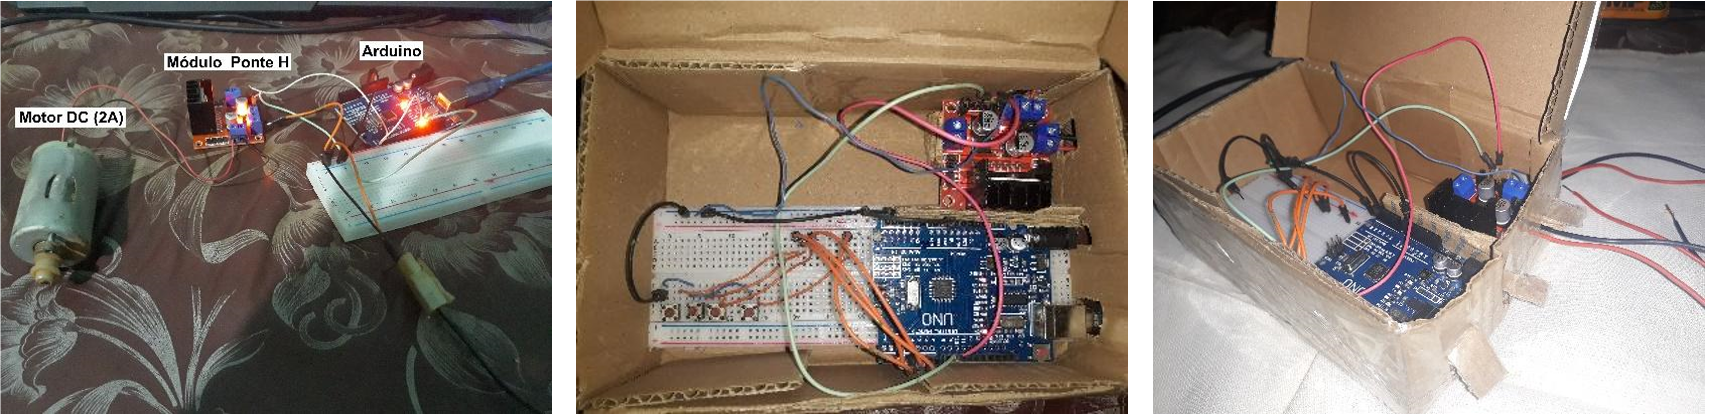
\includegraphics[width=1\textwidth]{imagens/CentralDeControleEsteira.png}
           \caption{Central de controle da esteira}
          \label{fig:CentralDeControleEsteira}
        \end{figure}
    
    Para um controle mais adequado da esteira, foi construído um painel. Este, é constituído de 4 pushbuttons, madeira e suportes plásticos para que os botões fiquem maiores e, consequentemente, mais fáceis de acionar, a Figura \ref{fig:PainelDeControlePrototipo} mostra o painel.
    
        \begin{figure}[h]
           \centering
           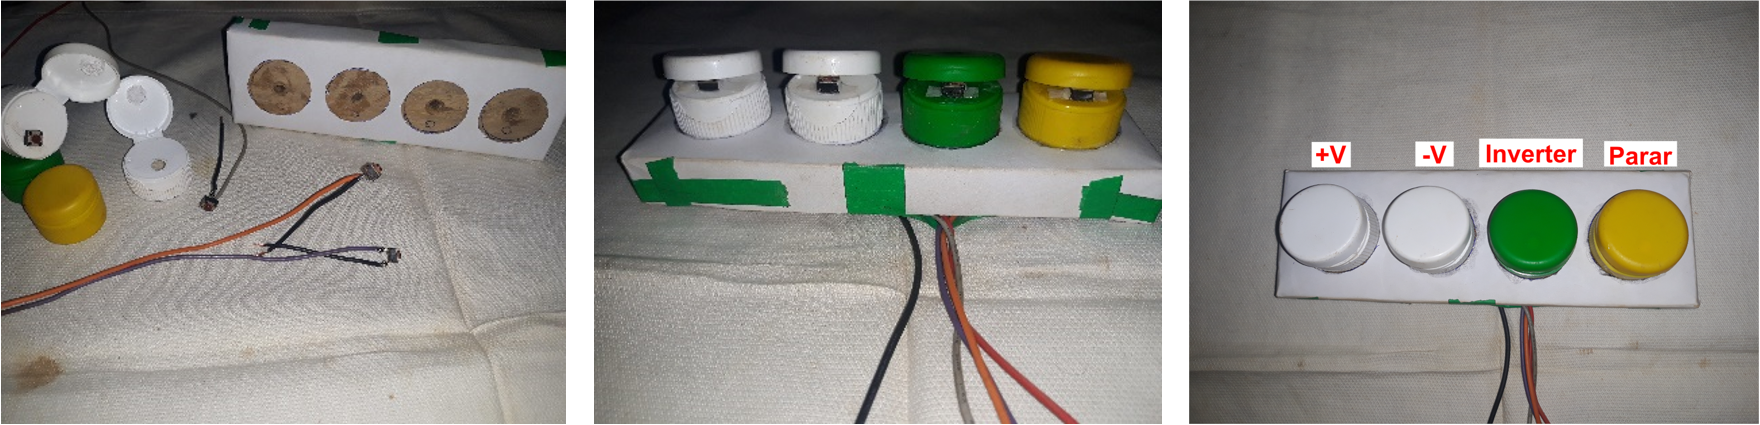
\includegraphics[width=1\textwidth]{imagens/PainelDeControlePrototipo.png}
           \caption{Painel de controle do protótipo}
          \label{fig:PainelDeControlePrototipo}
        \end{figure}
    
    


%\subsubsubsection{Montagem da esteira}
%\label{subsubsubsec_Montagem da esteira}



    Partindo para a construção do protótipo, nessa etapa, foi reutilizada a estrutura de uma esteira de ginástica. Além de reparos e limpeza, também foram feitas algumas adaptações para atendimento dos requisitos do protótipo, as principais foram:
    
    \begin{itemize}
        \item Fixação do motor do protótipo e correia especial. A correia e a engrenagem do motor realizam uma redução na pólia do rolete principal, isso gera mais torque na esteira. Também foi criado um esticador de correia no processo;
        \item Troca do tapete por um macio e compatível com a força do motor;
        \item Manutenção dos roletes que estavam travados e ajustes da tensão do tapete.
    \end{itemize}
    
    Dado que a estrutura é resistente, ela atende aos requisitos dos testes. A estrutura de fixação do kinect foi presa na esteira, em um local neutro (sem necessidade de ação do sensor). A Figura \ref{fig:prototipoEsteira} mostra o protótipo da esteira.
    
        \begin{figure}[h]
           \centering
           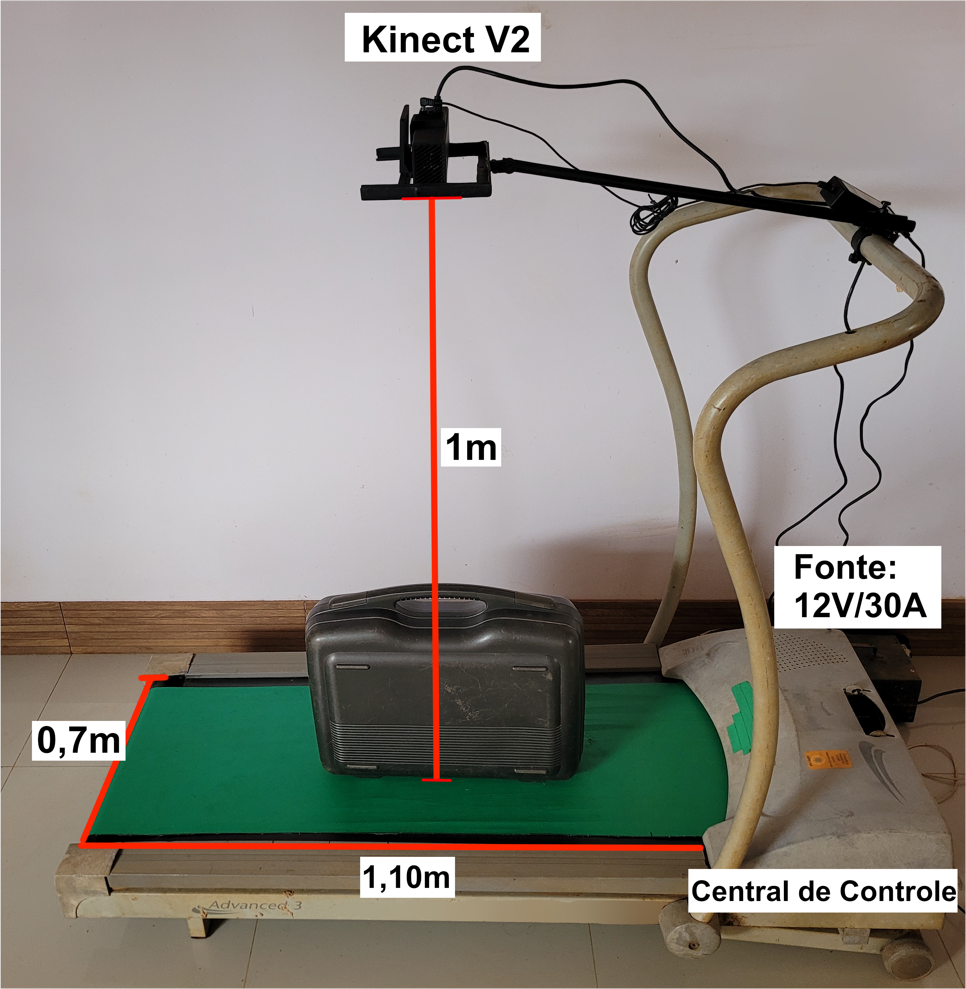
\includegraphics[width=0.5\textwidth]{imagens/prototipoEsteiraV5_.png}
           \caption{Protótipo do sistema com esteira e estrutura para posicionar o sensor}
          \label{fig:prototipoEsteira}
        \end{figure}

    Pela análise da Figura \ref{fig:prototipoEsteira}, é possível notar que a base do sensor está a 1 m de altura. O braço de fixação é móvel em três direções (cima, baixa e frente), isso foi utilizado para ajustes e testes quanto a altura do kinect, permitindo a configuração para até 1,5 m. A Figura \ref{fig:pointCloudDoAmbienteDaEsteira} mostra a visão do kinect do cenário de teste de forma estática e a Figura \ref{fig:pointCloudDaMala1_Roi1_Roi2} a \textit{point cloud} extraída com a amostragem móvel de uma mala.


        \begin{figure}[h]
           \centering
           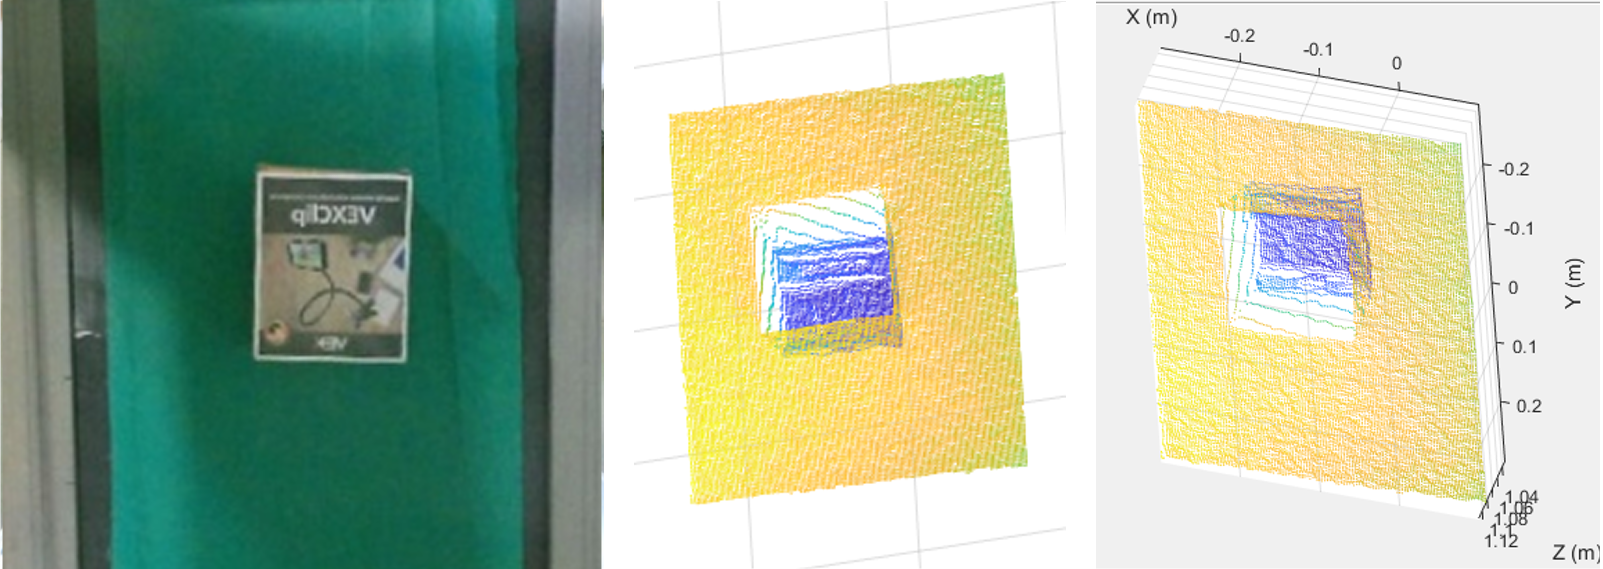
\includegraphics[width=0.6\textwidth]{imagens/pointCloudDoAmbienteDaEsteira_v2.png}
           \caption{\textit{Point cloud} do ambiente da esteira}
          \label{fig:pointCloudDoAmbienteDaEsteira}
        \end{figure}


%\subsubsection{Algoritmo para Amostragem de point cloud de forma móvel}
%\label{subsubsec_Algoritmo para Amostragem de point cloud de forma móvel}

    A captura móvel é realizada mediante alguns parâmetros, sendo eles um \textit{slice} (roi da captura), que define a região da \textit{point cloud} a ser coletada, passo de amostragem e frequência de amostragem. A partir disso, o sensor é posicionado na estrutura de fixação e a mala é movida pela região de ação do mesmo. Sendo assim, são realizadas N capturadas de \textit{point clouds}, os chamados \textit{slices}, para serem unidos formando uma \textit{point cloud} completa da bagagem. Com isso, a diferença desse método para o estático é a necessidade de realizar um tratamento mais extenso, consistindo em concatenar todas as amostras para formar a \textit{point cloud} final. O Algoritmo \ref{alg:Captura de Point Cloud movel} mostra a lógica seguida para aplicação dessa abordagem. A implementação desse algoritmo pode ser acessada no Apêndice \ref{apend_Códigos fonte do sistema de médida de bagagens}.


% \normalem %%%% disable auto underline

\begin{algorithm}[h!]
\caption{Captura de \textit{point cloud} móvel}\label{alg:Captura de Point Cloud movel}
\SetKwInOut{Entrada}{Entrada}
\SetKwInOut{Saida}{Saída}
\SetKwFor{Enqto}{enquanto}{faça}{fim enqto}
\SetKw{Retorna}{retorna}

\Entrada{O sensor Kinect $K$, o passo de amostragem $a$ em metros, a altura do sensor $h$, a região de interesse $r$ de captura e a tolerância $t$ de amostras para término}
\Saida{Nuvem de pontos (\textit{point cloud}) $P$}
\;
$P \gets \{\}$ \;
$f \gets$ \textbf{calcule} a frequência do sensor com base na amostragem $a$\;
\textbf{inicie} o sensor $K$ com a frequência $f$\\
$numpassos \gets 0$ \\
\Enqto{a tolerância $t$ de amostras sem objetos não for atingida}{
    $p \gets$ \textbf{leia} a point cloud do sensor $K$ \;
    $p_r \gets$ \textbf{retorne} somente os pontos na região $r$ de $p$ \;
    $p_m \gets$ \textbf{mova} os pontos $p_r$ na direção do eixo $y$ em $(numpassos * a)$ \;
    $P \gets P \cup p_m$ \Comment{concatena os pontos $p_m$ a \textit{point cloud} $P$}\;
    $numpassos \gets numpassos+1$\;
}
\Retorna $P$
\end{algorithm}

% \ULforem %%%% enable auto underline



    Pela análise do algoritmo é possível separar o processo de captura nos seguintes passos:
    
    \begin{enumerate}
        \item Definir parâmetros de entrada:
        \begin{enumerate}
            \item Passo de amostragem: depende da velocidade com que o objeto irá passar pelo sensor. Foi utilizado 5 cm e a opção 3 de velocidade (0,205 m/s);
            \item Roi: corresponde ao \textit{slice} de amostra, foi utilizado 5 cm de comprimento por 50 cm de largura;
        \end{enumerate}
        \item Realizar amostragem da point cloud:
        \begin{enumerate}
            \item Para cada amostra, concatenar a mesma em uma matriz de pontos resultante;
        \end{enumerate}
        \item Retorna a Point Cloud resultante.
    \end{enumerate}

    Como pode ser percebido na Figura \ref{fig:pointCloudDaMala1_Roi1_Roi2}, foi possível utilizar o método móvel para amostrar os pontos do objeto. 

        \begin{figure}[h]
           \centering
           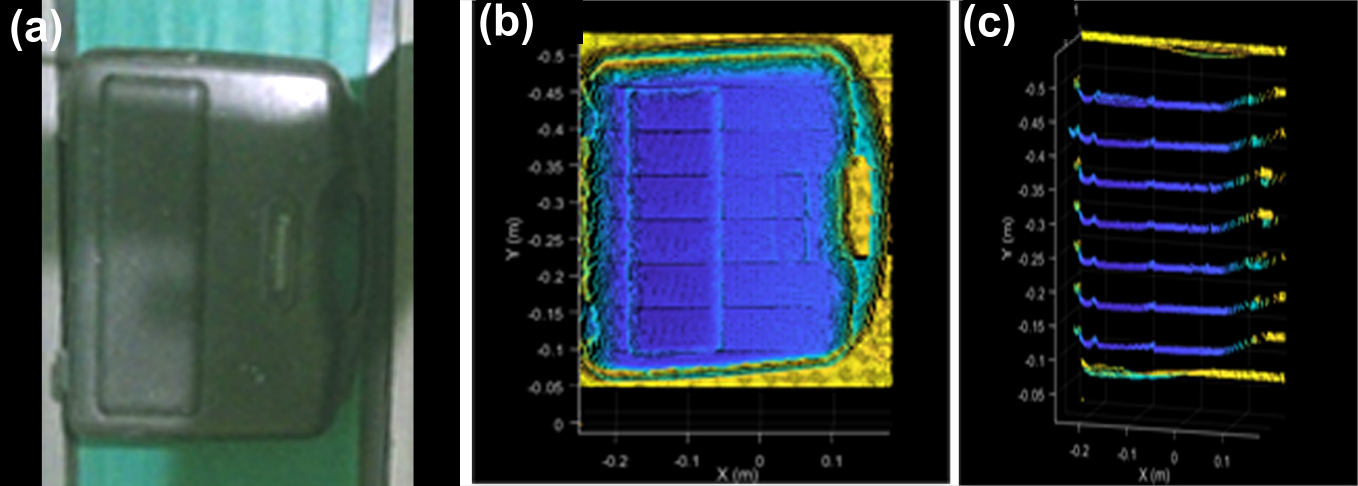
\includegraphics[width=0.7\textwidth]{imagens/pointCloudDaMala1_Roi1_Roi2_v2.png}
           \caption{\textit{Point cloud} da mala 1 e tamanho do slice por captura. (b) slice1 = 5 cm x 50 cm x 50 cm. (c) slice2 = 1 cm x 50 cm x 50 cm}
          \label{fig:pointCloudDaMala1_Roi1_Roi2}
        \end{figure}
    
    Nota-se que existem duas medidas para \textit{slices} (ROI). A Figura \ref{fig:pointCloudDaMala1_Roi1_Roi2}b tem um \textit{slice} de 5 cm x 50 cm x 50 cm, apresentando mais detalhes da bagagem, consequentemente, produzindo resultados mais precisos. Já a Figura \ref{fig:pointCloudDaMala1_Roi1_Roi2}c tem um \textit{slice} de 1 cm x 50 cm x 50 cm, coletando menos detalhes, porém reduzindo tempo de processamento e complicações como quando os pontos se sobrepõem entre dois passos. Contudo, para os testes foi utilizado o slice1 da  \ref{fig:pointCloudDaMala1_Roi1_Roi2}b, que retorna resultados mais precisos.
    
    
    
    

\section{Processamento da \textit{point cloud}}
\label{subsec_Processamento da Point Cloud}

    Na presente Seção será exposto o fluxo de tratamento da \textit{point cloud} desenvolvido para o protótipo, assim como a explicação de cada etapa adotada. Nesse caso, uma observação relevante é que o fluxo de tratamento inicial com Roi e segmentação é efetivo para trabalhar com a \textit{point cloud} em cenários menos exigentes. Isso é devido à precisão do Kinect, que não apresenta muitos ruídos (\textit{outliers}). No entanto, pode ocorrer pequenos desvios dos pontos por conta da reflexão natural do infravermelho na superfície da bagagem.
    
    Tendo em vista essa questão, mostrou-se interessante realizar uma filtragem para normalizar a posição dos pontos e retirar ruídos. Isso pode aumentar a exatidão das medidas. Outra vantagem é que, dada uma etapa de filtragem, pode ser desenvolvido um processo preparado para retirar outlier exagerados, como, por exemplo, pontos totalmente fora da bagagem. Sendo assim, a Figura \ref{fig:fluxoTratamentoPointCloudBagagens} ilustra o fluxo completo de tratamento da \textit{point cloud} desenvolvido na presente pesquisa. É importante destacar que o convex hull também foi ilustrado nesse fluxo dado que ele pertence à etapa de processamento.
    
        \begin{figure}[h]
           \centering
           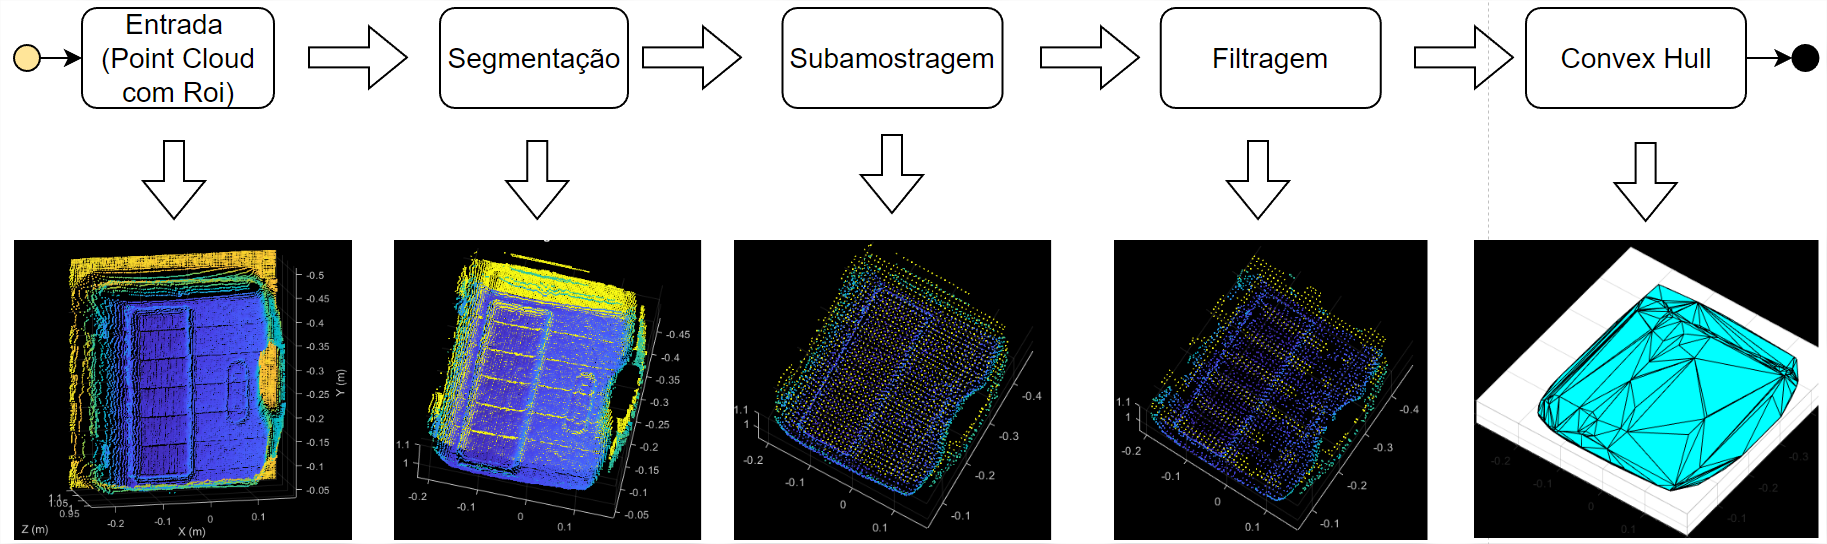
\includegraphics[width=1\textwidth]{imagens/fluxoTratamentoPointCloudBagagens.png}
           \caption{Fluxo de tratamento da \textit{point cloud} de bagagens para extração de dimensões slice = 5 cm x 50 cm x 50 cm}
          \label{fig:fluxoTratamentoPointCloudBagagens}
        \end{figure}
    
    O fluxo de tratamento consiste dos seguintes passos:
    
    \begin{enumerate}
        \item Entrada: Obter a \textit{point cloud};
        \item Segmentação: são filtrados os pontos de modo a descartar os que fazem parte da base da esteira;
        \item Subamostragem: consiste em filtrar a \textit{point cloud} reduzindo a densidade de pontos;
        \item Filtragem: é aplicado filtro de média na \textit{point cloud} de modo a normalizar a posição dos pontos;
        \item Convex hull: É utilizado para retornar os pontos de extremidade da mala, na Figura \ref{fig:fluxoTratamentoPointCloudBagagens} é mostrado por triangulação em azul para melhor visualização. 
    \end{enumerate}
    

    É interessante mencionar que esse tratamento adiciona uma tolerância ao sistema, permitindo que pequenos objetos próximos à bagagem sejam cortados da medida. Sendo assim, é interessante discutir sobre as principais etapas do fluxo que são a segmentação, subamostragem, filtragem e convex hull.


%\subsubsection{Segmentação}
%\label{subsubsec_Segmentacao}

    O processo de segmentação consiste em selecionar, da \textit{point cloud} de entrada, apenas os pontos que pertençam a um conjunto delimitado por uma constante de corte. Considerando a posição Top 90°, tem-se que a distância do sensor a base é uma constante conhecida. A partir disso é realizado um rastreio na \textit{point cloud} identificando e recuperando apenas os pontos que estão 5 cm acima do fundo. Ainda nesse processo, para cada ponto da mala, são adicionados pontos na altura da base em paralelo. Isso é feito para gerar o formato final do objeto e garantir um melhor resultado para o convex hull. Ou seja, sendo $P_i$ um ponto do conjunto de corte, é feita uma concatenação gerando uma \textit{point cloud} $P_r$.
    
    \commentBlock{
    
     \begin{equation} \label{eq:segmentacaoPtCloud}
        \begin{split}
            (\forall P_i \in conjunto\_de\_corte) P_r \gets \{P_r \cup P_i \cup (P_ix, P_iy, h)\}
        \end{split}
    \end{equation}
    
    }
    
    
    No presente modelo, a segmentação é um passo importante, dado que retira os pontos da base da esteira restando apenas os pontos da mala. Se a posição do sensor for alterada para, por exemplo, diagonal 45°, essa fase é o principal elemento do modelo que deve ser adaptado para possibilitar a aplicação dos outros passos de tratamento e a obtenção das dimensões. 
    
%\subsubsection{Subamostragem}
%\label{subsubsec_Subamostragem}   

    Já a subamostragem consiste em, dado um valor inteiro de passo, iterar sobre a \textit{point cloud} coletando os pontos que condizem com o mesmo. Para garantir um resultado uniforme que represente a mala original, é estabelecido a porcentagem mínima de pontos a serem retornados ao final da subamostragem. Esse processamento tem o principal objetivo de reduzir a quantidade de pontos a serem processados na medida. Ocasionalmente, podem ser retirados alguns \textit{outiliers} nessa lógica.


%\subsubsection{Filtragem}
%\label{subsubsec_Filtragem}

    A etapa de filtragem é a mais extensa, e consiste da aplicação de um filtro de distância média que descarta pontos fora dos limites da mala. Esse filtro é uma variação do conceito do DbScan, descrito na Seção \ref{subsec_Metodos para Clusterização}. No caso, é considerado um valor de distância de descarte (\textit{threshold}) e o número de vizinhos ($N$) que serão englobados para cada ponto $P_i$. Por padrão, esses números foram definidos como 1 e 3 respectivamente. 
    
    A partir desses dados é realizado um rastreio na \textit{point cloud}. Um ponto é considerado outlier quando o desvio padrão da distância média entre seus $N$ vizinhos mais próximos é maior que o threshold especificado. Tomando como referência a Figura \ref{fig:imagens/FiltragemPtCloud}, é indicado alguns outliers que são descartados da \textit{point cloud}. Também são ilustrados os dados de distância e número de vizinhos definido para o filtro.

        \begin{figure}[h]
           \centering
           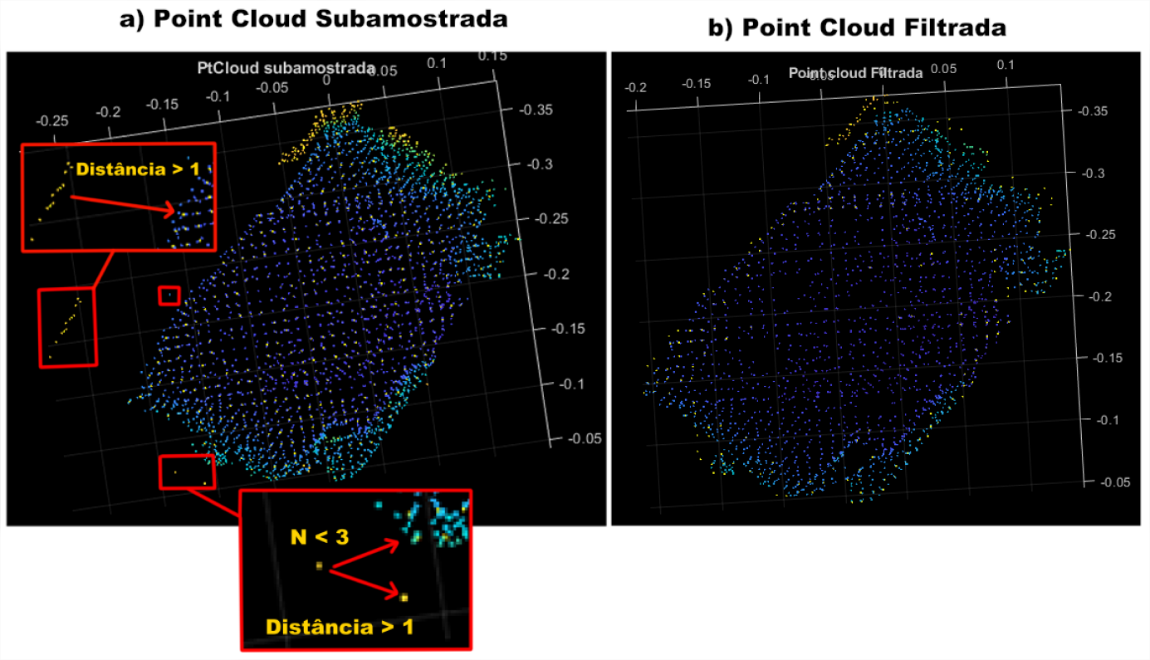
\includegraphics[width=1\textwidth]{imagens/FiltragemPtCloud.png}
           \caption{Filtragem de \textit{point cloud} de uma mala N = 3, threshold = 1}
          \label{fig:imagens/FiltragemPtCloud}
        \end{figure}

    É importante destacar que, os pontos descartados não correspondem a pontos de alças, rodas ou etiquetas. O intuito dessa etapa é apenas uniformizar a \textit{point cloud}, para melhorar a exatidão do modelo. Possíveis origens dos outliers ilustrados são os já mencionados reflexos do sensor nas superfícies, que, por vezes, não são retirados em etapas anteriores a filtragem. 
    
    Outra vantagem da filtragem é que pequenos objetos (ex. moeda, chave, batom, caneta) que possam ter caído na esteira e que não estejam anexados a bagagem, são cortados e não influenciam o resultado.

    
%\subsubsection{Convex hull}
%\label{subsubsec_Convex hull}    
    
    No final de todo o processo citado, é aplicado o convex hull para coletar os pontos de extremidades da \textit{point cloud} tratada. Esses pontos representam o menor polígono que reveste toda a superfície da bagagem. A partir disso já é possível obter dados quanto ao volume real, isso é, o volume que corresponde ao formato discretizado da mala.
    
    A etapa seguinte é o pós-processamento, que utiliza os pontos de hull para medir os valores de largura, altura e profundidade. A partir desses dados pode ser calculado o volume de armazenagem da bagagem na aeronave, que é em formato de paralelepípedo. Sendo assim, existem dois dados que podem ser utilizados para aprimorar o processo de check-in e despacho.
    
    
    
\section{Pós-processamento}
\label{subsec_Pos-processamento}

    Recapitulando, o desenvolvimento do sistema foi dividido em captura, tratamento de dados e extração de dimensões. Nessa Seção serão explorados os métodos criados para extração das dimensões da \textit{point cloud}. Segundo os dados da revisão sistemática, os algoritmos mais utilizados para esse fim são o convex hull e quadrados mínimos (MBB) \cite{guffanti_2020_the, gao_2018_minimum, chen_2013_research}.
    
    Nessa pesquisa foi utilizado o convex hull para extração do volume mais próximo ao formato da bagagem e obtenção dos pontos de extremidade. Já o OMBB foi utilizado para retornar as dimensões aproximando o formato a um paralelepípedo, fornecendo uma medida bem próxima do que é feito na prática dos aeroportos. Esse método também garante que, caso a mala esteja em outra posição, por exemplo, diagonal, seja possível calcular os dados baseada na orientação da \textit{point cloud}. 
    
    A abordagem adotada é inspirada no fluxograma ilustrado na Figura \ref{fig:fluxogramaOMBB}, dividido em 2 fases. Na primeira é aplicado o AABB, em sequência o resultado é manipulado para obter o OMBB, os seguintes detalhes podem ser pontuados:
    
    \begin{itemize}
    
        \item Fase 1: são retornados os dados dos limites x, y e z da \textit{point cloud} alinhado com os eixos. É importante salientar que a \textit{point cloud} de entrada já corresponde aos pontos do convex hull. Esse resultado consiste em um retângulo que tangência os limites máximo e mínimos da mesma;
        
        \item Fase 2: o resultado do passo 1 é rotacionado no sentido horário pelo uso de uma matriz de racionamento. A cada passo de rotação os pontos são movidos de modo a ajustar a área do retângulo ao formato da \textit{point cloud}, armazenando sempre o retângulo de menor área. Esse processo é repetido até todos os pontos de hull terem colidido ao menos uma vez com alguma extremidade das linhas do retângulo, então é retornado o retângulo de menor área que engloba os pontos, esse, corresponde ao OMBB.
        
    \end{itemize}
    
    A partir dos pontos de vértice do retângulo mencionado, é possível calcular a Altura, largura, profundida e volume do objeto de forma simplificada. Para tanto, é computado o módulo dos vetores entre os pontos de vértice das laterais desse retângulo, correlacionando esses dados com as informações de dimensões citadas.
    
    Essa lógica, consequentemente, aproxima qualquer objeto a um corpo em formato de caixa. Como mencionado, para obtenção do volume do objeto de maneira mais fiel ao formato da \textit{point cloud}, o método convex hull foi utilizado. 



